\documentclass{article}

\usepackage[margin=1.5cm, includefoot, footskip=30pt]{geometry}
\usepackage{amsmath}
\usepackage{amsfonts}
\usepackage{amssymb}
\usepackage{graphicx}
\usepackage{tikz}
\usetikzlibrary{positioning,calc}

\title{A Heterogeneous Moran Process for the Analysis of Public Goods Games}
\author{Harry Foster, Vince Knight, Sebastian Krapohl}
\date{\today}

\begin{document}
\maketitle
\section{Introduction}

\section{Literature Review}

Evolutionary game theory has long been at the forefront of the study of
emergent cooperation, showing how a strategy that is seemingly unfavourable for
the individual, but beneficial to the collective, can become dominant in
systems of rational actors. This is often shown through the study of games such
as the iterated prisoner's dilemma\cite{IPD1,IPD2} and the snowdrift
game\cite{Snowdrift1}. These examples, however, only allow for pairwise
interactions, which does not accurately represent many real-world scenarios.
Therefore, we look at a common game used to model the sharing of resources and
interactions between multiple people - the public goods game.\\

In order to further tailor the idea of a public goods game to real world
scenarios, we introduce the idea of heterogeneity to the system. Often in the
study of games we consider each individual to exist in the same conditions -
having the same utility and probability of transitioning to a different action
type. However, this does not accurately reflect many of the interactions that
occur in the real world, where individuals may have different factors affecting
which strategies they are able to take. For example, in a public goods game,
one player may wish to contribute \(x\) units to the public good, however they
do not have enough wealth available to spare such a contribution. Heterogeneity
allows us to give varying attributes to the different actors in order to
simulate such situations. These attributes can be encoded into the players
themselves as separate to the game, for example the reputation in \cite{Maa},
exist within the strategies of the players \cite{Lei, Flores}, or they may
exist within the actual payoffs which the players receive. We will look at
multiple different ways in which heterogeneity can be implemented in order to
model different scenarios.\\

In much of the literature, we see heterogeneous public goods game being played
graphically. By this I mean that in much research, players are placed on graphs
(often regular square lattices, as in \cite{Maa, Flores}) and participate in
multiple public goods games at the same time, with their payoff being the
combined payoff from all their games. This gives even more weight to the
decision to cooperate or defect, and allows players to interact in scenarios
with many different levels of these heterogeneous attributes. We also see many
ideas for what these attributes could be based upon. \cite{Maa} takes the idea
of that players could build a reputation through their decisions across
multiple generations, with players refusing to contribute higher amounts to
groups made up of those who have a reputation for defection. While this is a
dynamically updating heterogeneous attribute, some have proposed static
attributes based on inherent properties of the individuals, such as in
\cite{Lei} where the players participate in different amounts of games, and
contribute different amounts based on this factor.\\

In both of the above cases, it is shown that an increased scrutiny of
heterogeneous attributes in a spatial public goods game is beneficial to the
emergence of cooperation, though for different reasons. In \cite{Maa}, we see
that increasing such scrutiny obviously harms defectors, as they receive
reduced payoffs based on their low reputation due to being unable to coerce
high contributions from other players. \cite{Lei}, however, finds that if we
encourage players to cooperate with those in a similar number of games to them,
here done by tuning the \(\beta\) parameter, the high-degree defector nodes are
unable to gather a large payoff, and so will be unable to spread their
defection to their neighbours. If you encourage players to interact with those
with different degrees, however, then middle-degree defectors will make heavy losses and be unable to survive.\\

\cite{Flores} shows how the benefits of this heterogeneity are not always as
pronounced as it may seem. When the contribution is not calculated by some
attribute, but rather is an attribute in and of itself (essentially becoming a
new strategy) then even in systems where contribution dominates, we will see
low-value contributions act as a sort of defection against the most globally
beneficial strategies. Therefore, we can see that the emergence of cooperation
is not the end of the story in some cases, and we must look at what sort of
cooperation it is that we have fostered the emergence of.\\

One common theme in the spatial public goods game is the manner in which
cooperation spreads. An initial ``invasion" of defectors leads to cooperation
mainly existing within small clusters. These clusters, however, are much more
profitable than their defecting neighbours. Therefore, the cooperating clusters
will influence the nearby defectors to join in, which eventually spreads
throughout the system. This relies on the ability of the clusters to resist the
initial invasion of defectors - an occurrence which relies on a high enough
\(r\) value (the positive multiplier of the contribution to the public good).\\

We also see that a potential climate club may soon be forming within the
European Union. While it functions slightly differently to the classic example
in \cite{Climate Clubs}, it follows the same principles of encouraging
countries to join the group by punishing those outside of the club, in order to
attempt to reduce overall carbon emissions. This is the ``Carbon Border
Adjustment Mechanism" \cite{CBAM}. Currently, all goods within the EU require
taxation based on their carbon footprint, however imported goods from outside
cannot be subject to such taxes. CBAM aims to prevent foreign goods from
gaining benefits due to environmentally harmful practices by enforcing that EU
companies report the carbon content of imported goods, and purchase
certificates to cover the environmental cost of said goods. However, if a
country already levies a tax on their own goods (similar to the EU's carbon
tax), then this cost will be taken into consideration, and fewer certificates
must be purchased. This discourages the importation of goods from countries
which do not levy a similar tax on their own items, forming a structure which
behaves very similarly to the ``climate clubs" in \cite{Climate Clubs}.




\section{The Model}

\subsection{An Initial System}

In this section, we will look at the underlying model of the heterogeneous Moran process. We define the following:

\begin{itemize}
    \item \(N\) \textbf{ordered} individuals
    \item \(k\) types \(A_1, A_2, \dots A_k\)
    \item A state space S given by the set of ordered \(N\)-tuples with entries of type \(A_1, A_2, \dots A_k\). 
          Note that \(|S|=k^N\).\\
    A state \(v = (v_1, v_2, \dots) \in S\) is called \textbf{absorbing} if \(v_i = v_j\) \(\forall\) \(i,j \in \mathbb{N^+}\) : \(i,j \le N\), and the set of absorbing states is called \(S^\Gamma\)
    \item A strictly positive fitness function \(f:S \to \mathbb{R}^N\)
\end{itemize}

Let $h(v,u)$ denote the Hamming distance~\cite{Hamming_Distance} between two states \(v, u \in S\). We consider a Markov chain~\cite{Markov_Chain}, where for the transition $v = (v_1, v_2, \dots, v_N) \to u = (u_1, u_2, \dots, u_N)$, the 
transition probability is defined as follows:\\
\begin{large}
    \begin{equation}
        p_{v, u} = 
        \begin{cases}
            \frac{\sum_{v_i = u_{i^*}}{f(v_i)}}{\sum_{v_i}f(v_i)} & \text{if }h(v,u) = 1 \text{, differing at position }i^*\\
            0 & \text{if }h(v,u) > 1\\
            1 - \sum_{u \in S \setminus \text{\{v\}}}{P_{v,u}} & \text{if }h(v,u) = 0
        \end{cases}
    \label{eqn:Probability_Function}
    \end{equation}
\end{large}

Transitioning denotes something slightly different in the heterogeneous case of the Moran process as compared with the homogeneous. While we would traditionally say an \textit{individual} was removed and a new individual was generated to replace them, we must now say an individual's \textit{action type} was removed, and replaced with a new action type. This is because the individuals themselves are ordered in the heterogeneous Moran process, and possess certain attributes specific to themselves. Therefore, we cannot say that the individual themself is replaced, but rather that their action type is replaced.\\

The final case in (\ref{eqn:Probability Function}) corresponds to a transition from \(v\) to itself. 
This is possible when a given individual has their action type removed
and any other individual with the same type is chosen for duplication. A direct computation of $P_{v,v}$ is given by:
\begin{large}
\begin{equation}
    \frac{1}{N}\sum_{i=1}^{N} \frac{\sum_{v_j = v_{i}}{f(v_i)}}{\sum_{v_j}f(v_i)}
    \label{eqn:(2)}
\end{equation}
\end{large}
This would require at least \(N^2 + N\) calculations. 
However, we can observe that a transition of some sort must occur, and so we simply take the probability of not transitioning to any \textbf{different} state as \(P_{v,v}\).\\

An important case which proceeds from (\ref{eqn:Probability Function}) is that of a transition \(v \to u\) where \(u\) contains an individual of a \textit{type} not found in \(v\). For example, the transition (0,1) $\to$ (0,2). This would be forbidden by the intuition of a standard Moran process - i.e the new individual being the duplication of another individual in \(v\). However, we can see that the standard formula yields \(p_{v,u}\) = 0 because \(\nexists\) \(v_i \in V: v_i = u_{i^*}\). Following this, we see that (\ref{eqn:Probability}) also correctly gives us \(p_{v,u}\) = 0 for any \textbf{absorbing} \(v \neq u\).\\

This model allows for heterogeneity as we have a fitness function dependent on the individual, not dependent on the action taken. Therefore, we can give different individuals of the same action type a different fitness by passing different attributes to the fitness function itself. We will see examples of this in future sections.\\

As this forms a Markov chain, we can therefore define a transition matrix \(T\) for any given state space. This can be used to show the transition probabilities between any two given states, and therefore can be used to find the fixation probabilities for any given starting state by the following method:\\

Given a transition matrix \(T\), we can calculate the state distribution after \(k\) iterations of the Moran process using the formula \(T^k\)  \cite{Markov_Chain}. Therefore, as \(k \to \infty\), we will clearly acquire a distribution that tends towards the absorption probabilities for a given starting state, as the process will stabilise only if we enter an absorbing state (while subsets of \(S\) of states may have extremely high probabilities of transitioning to each other, the only way to have certainty of not transitioning away from a state or pair of states is to be in one of the previously defined absorbing states.)\\
Thus, our absorption probabilities starting at are given by the non-zero entries in the matrix \(\lim_{k \to \infty} T^k\)

\section{The General Heterogenous Public Goods Game}

\subsection{The Standard Model and Transformations}

In this section, we shall see how this model can be applied to the classical public goods game. In this game, individuals choose whether or not to contribute to a public resource pool. In the end, the total resource is multiplied by some factor \(r > 1\) and distributed equally between each player. This model often encourages a behaviour known as ``free-riding" \cite{Climate Clubs}, where players refuse to contribute to the pool and simply take the benefit provided by other individuals' contribution. The classic problem of a public goods game is to provide an environment where such free-riding is not a profitable strategy - or rather, is less profitable than contributing to the public good.\\

In our model, we can simulate a public goods game by providing the following payoff function:\\
\begin{large}
\begin{equation}
    \sigma(v_i) = \frac{r\sum_{j=1}^N{C_{v_j}}}{N} - C_{v_i}
    \label{eqn:General Model}
\end{equation}
\end{large}\\
(where \(C_{v_j}\) is the contribution by individual j.) 

In the homogeneous public goods game, we can see that \(C_{v_j}\) can only take one of two values: some constant \(\alpha \) if individual j cooperates, and 0 if not. However, the heterogeneous game will require a more tailored \(C_{v_j}\).\\

Note that \(\sigma(v_j)\) can be negative which would then not lead to sensible probability values as needed in~\ref{eqn:Probability Function}. Therefore, we must look at some transformation of \(\sigma\) to use as our fitness function.\\

A common method \cite{Nowak 2006} for this is to apply the exponential function to our payoff function. By using \(e^{\kappa \sigma}\) as our fitness function we will have positive values, however this particular approach  gives:

\begin{large}
    \begin{equation}
        \frac{\sum_{v_i = u_{i^*}}{e^{\frac{\kappa r\sum_{j=1}^N{C_{v_j}}}{N} - C_{v_i}}}}{\sum_{v_i}e^{\frac{\kappa r\sum_{j=1}^N{C_{v_j}}}{N} - C_{v_i}}}
    \end{equation}
\end{large}\\

Now, as \(e^r\) does not rely on \(v\), we can take this out of the sum and acquire the following:

\begin{large}
    \begin{equation}
        \frac{e^{\frac{\kappa r\sum_{j=1}^N{C_{v_j}}}{N}}\sum_{v_i = u_{i^*}}{e^{ - C_{v_i}}}}{e^{\frac{\kappa r\sum_{j=1}^N{C_{v_j}}}{N}}\sum_{v_i}e^{-C_{v_i}}} = \frac{\sum_{v_i = u_{i^*}}{e^{ - C_{v_i}}}}{\sum_{v_i}e^{-C_{v_i}}}
    \end{equation}
\end{large}\\

and we see that in this case, \(p_{v,u}\) would not rely on \(r\). 
Therefore, let us consider some other methods of guaranteeing a positive fitness function.\\

The first of these is known as the "shifted linear" transformation. We take, for some small tunable \(\epsilon\):
\begin{large}
    \begin{equation}
        f(v_i) = \sigma(v_i) - \min_{v_j \in v} \sigma(v_j) + \epsilon
    \end{equation}
    \label{eqn:Shifted_linear}
\end{large}
This guarantees a positive value, with the lowest fitness taking the value \(\epsilon\), a parameter that can be chosen based on the system in question.\\

Another type of mapping that we can use is the ``Affine-linear mapping". In
this, for some tunable \(\epsilon\), we take the following:

\begin{large}
    \begin{equation}
        f(v_i) = 1 + \epsilon\sigma(v_i)
    \end{equation}
    \label{eqn:Affine-linear}
\end{large}\\




\subsection{The Homogeneous Case}
The most common type of public goods game is the homogeneous public goods game.
In this game, we consider that we have a constant \(C_{v_i} = \alpha\) for all players \(v_i\).
In this case, we take the payoff function:
\begin{large}
    \begin{equation}
        \sigma(v_i) = \frac{r\sum_{j=1}^N{k_j\alpha}}{N} - k_i\alpha = (Kr-k_i)\alpha
    \end{equation}
    \label{eqn:Homogeneous_fitness}
\end{large}\\
Where \(k_j = 1\) if j contributes and 0 if not, and \(K\) is the fraction of the population who contribute.\\

However, we cannot use \ref{eqn:Shifted_linear} transformation or else we once again run into a problem with too many factors cancelling down and becoming unreliant on \(r\):

\begin{large}
    \begin{equation}
        \begin{split}
        (K * r - k_i)\alpha - \min_j(K * r  - k_j)\alpha + \epsilon 
        = (1 - k_i)\alpha + \epsilon = \begin{cases}
            \epsilon & \text{if \(v_i\) contributes}\\
            \alpha + \epsilon & \text{if not}
        \end{cases}
        \end{split}
    \end{equation}
    \label{eqn:Homogeneous_fitness}
\end{large}\\

Not only does our choice of \(\epsilon\) become too powerful, but also we cancel out all reliance on \(r\)\\

Therefore, we take the affine-linear mapping shown in \ref{eqn:Affine-linear} in order to see our fixation probabilities.

We will begin by looking at the state space with \(N=4\) and see how cooperation emerges based on different values of \(r \text{ and } \alpha\).

%\begin{figure}[!h]
    %\centering
%\includegraphics[width=1\linewidth]{./Figures/%Homogeneous_Fixation_Probabilities_r_alpha/Main.png}
 %   \caption{Fixation probabilities in the homogeneous case. Here we take }
  %  \label{fig:Homogeneous_Fixation_Probability_r_alpha}
%\end{figure}

Here we can see how the various parameters can be tuned to affect our fixation
probabilities. As r increases, we see an increase in cooperation as individuals
benefit more from their own contributions. However, as \(\alpha\) increases,
individuals must pay more to contribute to the public good, which also benefits
defectors who receive higher payoffs without risking their own contribution -
leading to a wider gap between the payoffs of cooperators and defectors in the
game.\\
\newpage
\section{Public Goods Games with Heterogeneous Returns}

When we look at a public goods game, we often generalise the players to all
contribute the same amount. However, in the real world this is often not the
case, as different individuals may have different attributes which affect their
ability to contribute as much as others. In this section, we look at how a
heterogeneous population with respect to contribution can affect the fixation
probability.\\

We begin by defining a maximum value \(M\), which is the total contribution to
the public good in the case that all players contribute. The responsibility for
the contribution of such \(M\) is then split between all players according to
some rule. This rule will take the form of some \(\lambda\), such that
\(\sum_{j=1}^{N} j\lambda = M\).\\
 We look at 6 such rules for sharing the contribution between all players.

\subsection{The Linear Case}

In this case, players simply contribute an amount equal to their position
within the state. For example, a state (1,1,0,1) for \(M=10\) will
contribute (1, 2, 0, 4) respectively. For a given \(N, M\), we have that here,
\(\lambda = \frac{2M}{N(N+1_)}\)




\section{The Dirichlet Distribution}

\subsection{The Basics}

We begin with a beta distribution. Imagine you have tossed a coin \(N\)
times, observing \(H\) heads and \(T\) tails. Our beta distribution takes
two parameters: \(\alpha\) and \(\beta\) with values \(H+1\) and \(T+1\)
respectively. The "peak" (mode) of the beta distribution occurs at
\(\frac{H}{H+T}\).\\

Now the Dirichlet distribution extends this problem into \(K\) components.
Imagine you have a bag containing different coloured balls - red, blue, and
green. After a certain number of samples, you observe \(R\), \(B\), and \(G\)
balls of each colour respectively. Then, similarly to our beta distribution,
our dirichlet distribution takes the values \(\alpha_1 = R+1, \alpha_2 = B+1,
\alpha_3 = G+1\).\\
Now, unlike the beta distribution, the Dirichlet distribution
returns a vector of probabilities \(X = (x_1, x_2,...,x_K)\) such that
\(\sum_{i=1}^K x_i = 1\), rather than a single probability. While theoretically
the beta distribution can be used to return a probability vector which sums to
1 by taking the compliment of it's value for a given parameter (in our above
example, it could return [\(\frac{H}{H+T}, \frac{T}{H+T}\)]), the distribution
is not often used this way. For the Dirichlet distribution, we always obtain
such a vector. The PDF is therefore defined by this vector as follows:
\begin{large}
    \begin{equation}
        f(x_1, ..., x_k, \alpha_1, ..., \alpha_k) = \frac{1}{B(\alpha_1, \alpha_2, ...)}\Pi_{i=1}^K x_i ^ {\alpha_i}
    \end{equation}
\end{large}
where \(B(\alpha_1, \alpha_2,...)\) is the normalisation function
\begin{equation}
    \frac{\Pi_{i=1}^K \Gamma(\alpha_i)}{\Gamma(\sum_{i=1}^K \alpha_i)}
\end{equation}
and \(\Gamma\) is the Gamma distribution. This exists to ensure that
\(\int_{-\infty}^{\infty} f(x_1, ..., x_k, \alpha_1, ..., \alpha_k) = 1\)\\

Now let us look at the expected value of the Dirichlet distribution. We have the following:\\
\begin{large}
\begin{equation}
    E(X_i) = \frac{\alpha_i}{\sum_j \alpha_j}
\end{equation}
\end{large}
So as \(\sum_{j=1}^{K}\alpha_j = n\), we have that if we take a Dirichlet
distribution \(D_1\) with parameters \( (\alpha_1, \alpha_2, ...)\) and another
\(D_2\) with parameters \( (z\alpha_1, z\alpha_2, ...)\) for a constant \(z\),
they will retain the same mean for each component due to the following:
\begin{large}
\begin{equation}
    E(D_{2,i}) =
\frac{n_i}{n} = \frac{z\alpha_i}{\sum_{j=1}^{K}z\alpha_j} = \frac{\alpha_i}{\sum_{j=1}^{K}\alpha_j} = E(D_{1,i})
\end{equation}
\end{large} 

Now, as our number of observations \(n\) increases, we get that our expected
value converges to \(\frac{n_i}{n}\), where \(X_i\) is observed \(n_i\) times.
The variance of the data also behaves in a similar way. The explicit formula is
given by:

\begin{large}
\begin{equation}
    Var(X_i) = \frac{\frac{\alpha_i}{\sum_{j=1}^K \alpha_j}(1-\frac{\alpha_i}{\sum_{j=1}^K \alpha_j})}{\sum_{j=1}^K \alpha_j + 1}
\end{equation}
\end{large}

which tends to \(\frac{x_i(1-x_1)}{n}\) as \(n \to \infty\). We see that this
is the result that we would intuitively expect by normal statistical methods.
We also notice that as this is strictly decreasing as \(n \to \infty\), and so
we would acquire the result that \(Var(D_{2_i}) < Var(D_{1,i})\). This fits
with our intuition once again, as if we obtain more data for each case in the
same ratio (so for example, having data (2 red, 3 blue, 1 green) and then
obtaining the additional data (4 red, 6 blue, 2 green)), we will retain the
same mean value in our posterior distribution, however our variance will be reeduced.

\subsection{A Visual Example of Sampling from the Dirichlet Distribution}

Now for a deeper look into sampling from the Dirichlet distribution. Consider
each case as a vertex on the probability simplex as follows (we take K=3 as an
example, however we would consider a K-sided simplex for a Dirichlet
distribution with K components):

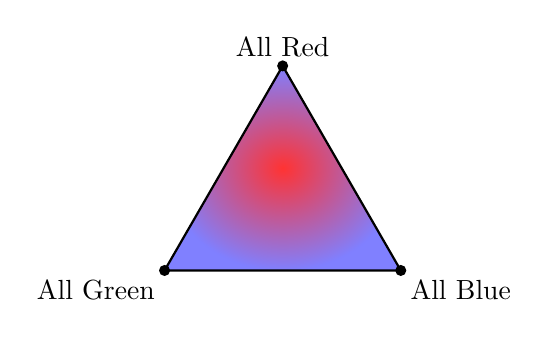
\begin{tikzpicture}

  \coordinate (A) at (0,0);
  \coordinate (B) at (3,0);
  \coordinate (C) at (1.5,2.598076211353316);


  \shade[shading=radial,
         inner color=red!80,
         outer color=blue!50]
         (A) -- (B) -- (C) -- cycle;



  \draw[thick] (A) -- (B) -- (C) -- cycle;

  \fill (0, 0) circle (2pt);
  \fill (3, 0) circle (2pt);
  \fill (1.5,2.598076211353316) circle (2pt);

  \node[below left]  at (A) {All Green};
  \node[below right] at (B) {All Blue};
  \node[above]       at (C) {All Red};

\end{tikzpicture}

The points on this simplex correspond to different probability vectors, with
the vertices representing the extreme cases in which our vectors are simply 1
for some entry, and 0 elsewhere. The distribution gives us which regions of the
simplex have a higher probability of being the true values (for example, 5 red,
4 blue, 4 green being in the bag). This is a visual description of the PDF of
the K-dimensional Dirichlet distribution.\\

Now how do the \(\alpha\) parameters control the spread of probabity across the
simplex? Well, as proven in the last section, we know that the ratio between
the \(\alpha s\) determines the expected value of the distribution, and the
total of the \(\alpha s\) determines the variance of the distribution. Thus, we
can picture the effects of the \(\alpha\) parameters visually as follows:

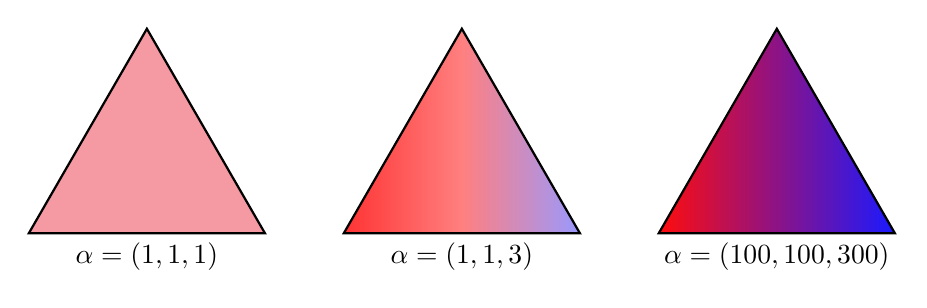
\begin{tikzpicture}[scale=1]


\def\shiftone{0}
\def\shifttwo{4.2}
\def\shiftthree{8.4}



\coordinate (A) at (0,0);
\coordinate (B) at (3,0);
\coordinate (C) at (1.5,2.598);
\begin{scope}
  \fill[red!90!blue!40] (A) -- (B) -- (C) -- cycle; 
  \draw[thick] (A) -- (B) -- (C) -- cycle;
  \node[below] at ($(A)!0.5!(B)$) {$\alpha = (1,1,1)$};
\end{scope}


\coordinate (A1) at (4,0);
\coordinate (B1) at (7,0);
\coordinate (C1) at (5.5,2.598);
\begin{scope}[shift={(\shifttwo,0)}]
  \path[shade, shading=axis,
        top color=red!80,
        bottom color=blue!40,
        middle color=red!50,
        shading angle=90]
        (A1) -- (B1) -- (C1) -- cycle;
  \draw[thick] (A1) -- (B1) -- (C1) -- cycle;
  \node[below] at ($(A1)!0.5!(B1)$) {$\alpha = (1,1,3)$};
\end{scope}


\coordinate (A2) at (8,0);
\coordinate (B2) at (11,0);
\coordinate (C2) at (9.5,2.598);
\begin{scope}[shift={(\shiftthree,0)}]
  \path[shade, shading=axis,
        top color=red!95,
        middle color=blue!60,
        bottom color=blue!90,
        shading angle=90]
        (A2) -- (B2) -- (C2) -- cycle;
  \draw[thick] (A2) -- (B2) -- (C2) -- cycle;
  \node[below] at ($(A2)!0.5!(B2)$) {$\alpha = (100,100,300)$};
\end{scope}

\end{tikzpicture}

Where the red regions represent areas of high probability, and blue regions are
those of low probability. We see that each \(\alpha\) corresponds to a
different vertex on the probability simplex, with the distribution being
concentrated towards a vertex depending on it's corresponding \(\alpha\) value.
To illustrate the reason behind this, consider a set of \(\alpha\)s where
\(\alpha_i = 0 \forall i \neq 1, \alpha_1 = 1\). In this case, our probability
would be entirely concentrated on the vertex corresponding to \(\alpha_1\),
with no variance. This is obvious from the expected value formula above. In a
similar case of \(\alpha_i = 1 \forall i \neq 1, \alpha_1 = 100\), we would see
a very heavy concentration of probability towards the vertex corresponding to
\(\alpha_1\), however we would not see it entirely concentrated into one point
as before, instead there would be some variance, who's source is the other
non-zero \(\alpha\) values, that causes the probability to become more
distributed across the simplex.\\

This illustration shows how the \(\alpha\)s affect the probability distribution
in practice, and serves as a visual demonstration of how the formulas in the
previous section behave. Now, we shall move on to look at how the Dirichlet
distribution applies in practice to our public goods game.

\subsection{The Dirichlet distribution and a Markov Process}

Consider now a Markov process. For a transition matrix \(T\), \(T_{A,B} =
p_{A,B}\), the probability of transitioning from state \(A\) to state \(B\) (in
this example, we have ordered the states in our state space, and \(A,B\) are
integers). When we look at the the steady state of a given transition
matrix, we are left with the vector \(\textbf{\(\mu\)} = (\mu_1, \mu_2, ...)\), where once
the steady state is reached, \(\mu_i\) gives the proportion of time steps that,
on average, will be spent in state \(i\). This is an eigenvector for \(T\).
This is because for any state distribution vector \(\tilde\mu\), we have that
\(\tilde\mu T\) gives us the probability of being in each state at the next
timestep. For the vector \textbf{\(\mu\)}, we get
\(\textbf{\(\mu\)}T=\textbf{\(\mu\)}\).\\

Now, upon obtaining this vector for a given Markov chain, we can see the
folllowing properties:

\begin{itemize}
    \item The entries of \textbf{\(\mu\)} are positive
    \item The sum of the \(\mu_i\)s is equal to 1
\end{itemize}

Now, these probabilities can be meaningfully interpreted as the realisations of
components of a Dirichlet distribution. Therefore, we can say that
\(\textbf{\(\mu\)} \sim Dirichlet(\alpha_1, \alpha_2, ..., \alpha_{k^N})\). Now, if
we have fixed probabilities for the entries of a given transition matrix \(T\),
then the \textbf{\(\mu\)} that we obtain is the average proportion of time
steps spent in each state. Thus, we can say that the obtained vector
\(\textbf{\(\mu\)} = E(X) = (E(X_1), E(X_2), ...)\), where \(X\) is a random
variable with a Dirichlet distribution. We can therefore fit a Dirichlet
distribution according to this.\\

In the case of a heterogeneous moran process, our steady state is trivial - we
always remain in one of the absorbing states \(v \in S^{\Gamma}\). Therefore,
for any given starting state, we have that our \textbf{\(\mu\)} only has
non-zero entries for \(\mu_i\)s corresponding to absorbing states. This means
that we would model this Dirichlet distribution with many \(\alpha_i = 0\)
(specifically all but \(k\) entries of \textbf{\(\mu\)} are equal to 0).
However, as the Dirichlet distribution is parameterised by strictly positive
\(\alpha\) values, we omit these and simply write \textbf{\(\mu\)} with only
the entries according to their absorbing states. In this case, our
\textbf{\(\mu\)} corresponds with the probability of entering each absorbing
state in a given markov process.\\

For the case of introspection dynamics, we have a more standard interpretation
of \textbf{\(\mu\)} as described before, where \textbf{\(\mu\)} corresponds to
the average number of timesteps spent in each state once we have reached the
steady state of the process. Now, given this case, let us look further into how
this works with regards to a certain type of heterogeneity - that being where
the attributes of each player are assigned according to a random variable
\(H\). In this case, the transition probabilities \(T_{A,B}\) are some function
\(t(H)\). Then, we must look at \textbf{\(\mu\)} in this context as a
random vector.\\

%TODO - look deeper into eigenvectors of random matrices. I think we may end up
%being able to say that as we simulate more and more, then \textbf{\(\mu\)} will
%tend to the expected value of the distribution where each player has the
%expected value of each attribute. This is homogeneous if everyone is using the
%same distribution, and not homogeneous if not.\\

%Also find citations for the Dirichlet distribution work and random markov
%chains.
%https://mast.queensu.ca/~communications/Papers/msc-jiayu-lin.pdf?utm_source=chatgpt.com
%looks good for Dirichlet distributions.





\newpage
\begin{thebibliography}{9}
\bibitem{IPD1}
Vince Knight, Marc Harper, Nikoleta Glynatsi et al (2024) - Recognising and evaluating the effectiveness of extortion in the Iterated Prisoner’s Dilemma
\bibitem{IPD2}
Robert Axelrod (1980) - Effective Choice in the Prisoner’s Dilemma
\bibitem{Snowdrift1}
Zhenyu Wang, Nigel Goldenfeld (2011) - Theory of cooperation in a micro‑organismal snowdrift game
\bibitem{Maa}
Xiaoiian Maa et al (2021) - Effect of reputation-based heterogeneous investment on cooperation in spatial public goods game
\bibitem{Lei}
Chuang Lei et al (2010) - Heterogeneity of allocation promotes cooperation in public goods games
\bibitem{Flores}
Lucas S. Flores et al (2023) - Heterogeneous contributions can jeopardize cooperation in the public goods game
\bibitem{Hamming_Distance}
Dave K. Kythe, Prem K. Kythe (2012) - Algebraic and Stochastic Coding Theory
\bibitem{Markov_Chain}
William J. Stewart (2009) - Probability, Markov Chains, Queues, and Simulation: The Mathematical Basis of Performance Modeling
\bibitem{Climate Clubs}
William Nordhaus (2015) - Climate Clubs: Overcoming Free-riding in International Climate Policy
\bibitem{Nowak 2006}
Martin A. Nowak (2006) - Evolutionary Dynamics: Exploring the Equations of Life
\bibitem{CBAM}
Regulation (EU) 2023/956 of the European Parliament and of the Council of 10 May 2023 establishing a carbon border adjustment mechanism (Text with EEA relevance)
\end{thebibliography}


\end{document}